\begin{center}
  \begin{tabular}{rp{6cm}lp{12cm}}%{rl}
  % after \\: \hline or \cline{col1-col2} \cline{col3-col4} ...
  论文地址:& \href{https://arxiv.org/abs/1810.10866}{https://arxiv.org/abs/1810.10866} \\
  slides:& \href{http://yunshengb.com/wp-content/uploads/2017/03/nips_2018_r2l_workshop_talk.pdf}{{\footnotesize Convolutional Set Matching for Graph Similarity}}\\
  关键词:& \textbf{Graph Similarity, GCN, CNN} \\
  写于:& \date{2020-10-10}
  \end{tabular}
\end{center}

该论文\cite{bai2018convolutional}主要解决的问题是:给定两个图$\mathcal{G}_1, \mathcal{G}_2$,计算它们的相似性。图相似性计算是图数据搜索中的难点和核心点,由于图的同构性,衡量两个图的相似性是NP-hard问题。论文中提出了GSimCNN(Graph  Similarity Computation via Convolutional Neural Network)来解决这个问题。

\textbf{GSimCNN思路}\hspace{12pt}该方法使用了图像识别中CNN的方法,通过GCN可以得到每个graph的多个结点特征矩阵(GCN有几层就有几个节点特征矩阵),这样就得到了$\mathcal{G}_1, \mathcal{G}_2$的节点特征矩阵,再根据这两个结点特征矩阵构造一个相似矩阵(Similarity Matrix),构造方法是从$\mathcal{G}_1, \mathcal{G}_2$各取一个结点的特征矩阵做内积得到相似矩阵中的一个元素。如果GCN有k层,则可以得到k个相似矩阵。在经过CNN的一顿操作后将CNN的输出输入到一个全连接的MLp中,得到两个graph的相似度分数。损失函数是均方误差损失函数(对于$\mathcal{G}_1, \mathcal{G}_2$,会有一个实际的相似度分数)。可参考Fig.\ref{fig:GSimCNN}。

\begin{figure}[h]
	\centering
	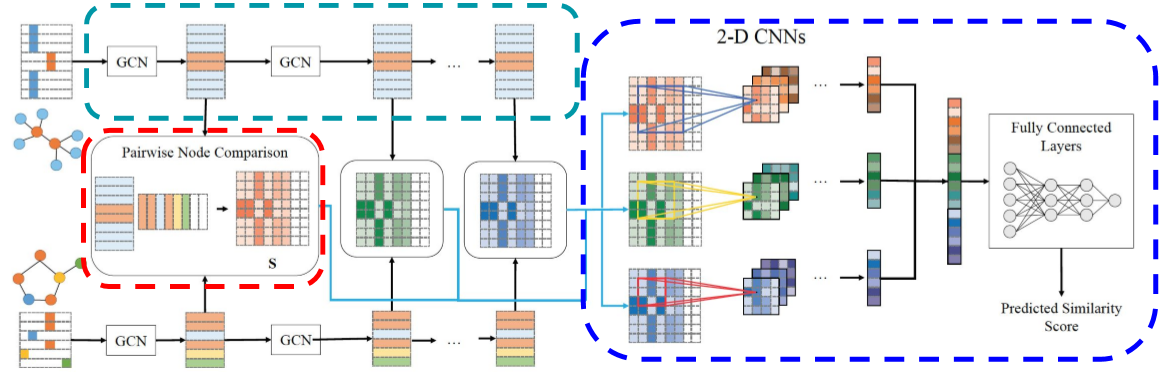
\includegraphics[width=.8\textwidth]{pics/GSimCNN.PNG}
	\caption{GSimCNN的三个阶段,分别用不同颜色的虚线框圈出}
	\label{fig:GSimCNN}
\end{figure}

如Fig.\ref{fig:GSimCNN}所示,是使用GSimCNN计算两个图相似性的过程,不同颜色代表算法的不同阶段。

{\textcolor[RGB]{64, 177, 189}{\textbf{Stage 1}}}\hspace{12pt}GCN阶段,使用一个多层的GCN为$\mathcal{G}_1, \mathcal{G}_2$中的每个结点生成表征,这样在GCN的每一层,都能够生成两个两个结点特征矩阵。若GCN有k层,则会有k对个结点特征矩阵对。{\color{red}为什么要在每一层计算一个相似矩阵呢?}因为GCN是基于汇集邻居的信息来表征的,第k层相当于汇集了k-hop的邻居的信息,而图的结构相似往往是局部的,而且是在不同尺度(图的规模)上的。而不同层的结点表征相当于代表了不同尺度的结构,也就能在不同尺度上进行图的相似性比较。  

{\color{red}\textbf{Stage 2}}\hspace{12pt}使用每一层的结点特征矩阵对,通过内积运算得到一个相似矩阵。因为GCN有k层,则会得到k个相似矩阵。

{\color{blue}\textbf{Stage 3} }\hspace{12pt}基于{\color{red}Stage 2}得到的k个相似矩阵,使用多个卷积核(Fig.\ref{fig:GSimCNN}中使用了3个2-D卷积核)来对多个相似矩阵进行卷积,最后将多个卷积核的结果向量进行拼接,输入到全连接的MLP中计算相似度分数。

在实验方面,作者使用了两类的baseline,一类是基于组合优化的近似GED(Graph  Edit Distance,相关论文表明当图地结点超过16时,GED将变得难以计算\cite{arora2019exact},因此也产生了很多近似算法)的算法,另一类的基于神经网络的算法。在这些算法中,GED的算法作为基准,其mse是0,但是复杂度太高,时间成本太高,GSimCNN与其他算法相比在mse和时间上都取得较好的效果。

论文中还有一些其他细节的处理,比如:对于不同大小的图的特征矩阵会进行padding,针对结点的排序使用了\cite{you2018graphrnn}的BFS的思路等。

至于论文的题目中的\textbf{set matching},因为沦为中使用的是Set matching的思路来计算两个图的相似性,一个图的所有结点的表征就是一个set。那为什么不适用graph-level的表征来直接计算图的相似性呢?(在论文的实验比较中有几个方法使用的就是graph-level的表征,如:EmbAvg, GCNMean, GCNMax,这几个方法在通过结点表征得到图表征时的方法不一样,如算术平均结点的表征作为图表征等)论文中给出的原因如下:
\begin{itemize}
	\item 没有使用更细粒度的结点表征
	\item 忽略了图级的交互(原文是{\color{red}{graph level interaction}},但不确定是什么意思)
\end{itemize}
也正是因为以上原因,论文将图相似性以set matching的角度来解决。个人认为论文是在更细粒度对两幅图的相似性进行了比较({{\color{red}{能否进行更细粒度的比比较呢?}}比如利用结点的属)。

论文中对GSimCNN得到的相似矩阵进行了可视化,发现相似或很不相似的图的相似矩阵都有一些明显的特点,如Fig.\ref{fig:sim}所示:
\begin{figure}[h]
	\centering
	%\hspace{1.5pt}
	\subfigure{
		\begin{minipage}{0.95\linewidth}
			\centering
			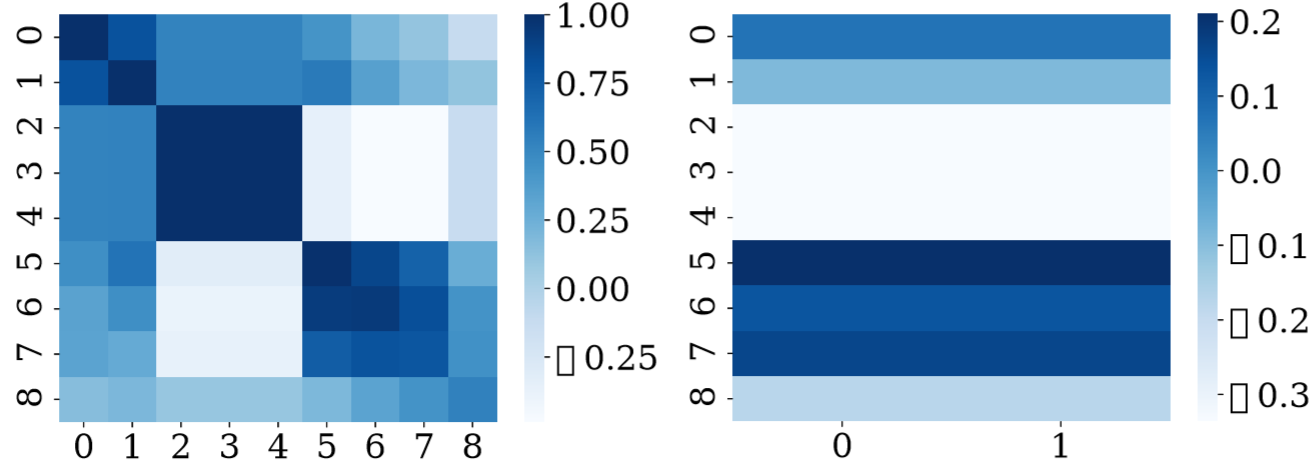
\includegraphics[width=.85\textwidth]{pics/sim1.PNG}
			\vspace{12pt}
			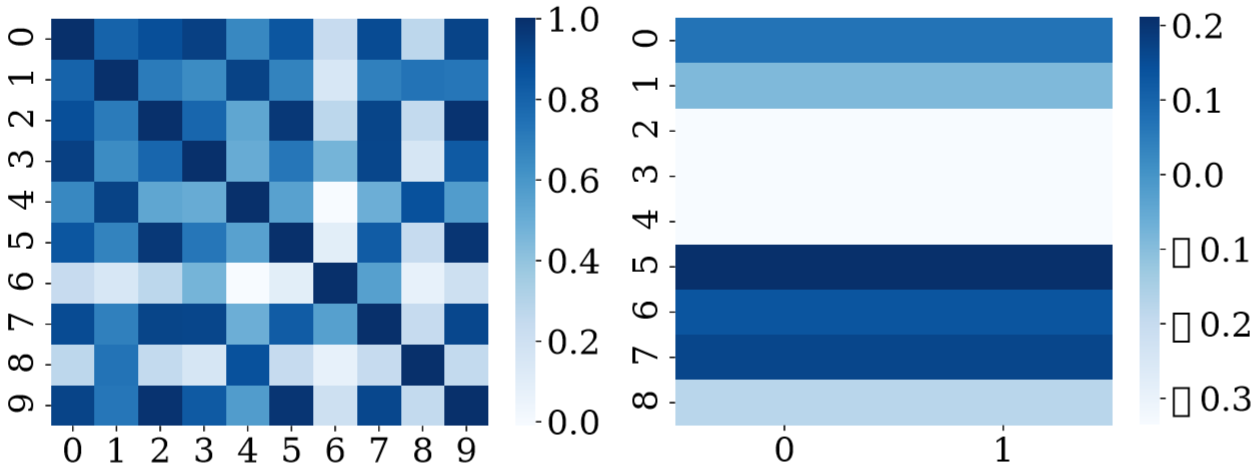
\includegraphics[width=.85\textwidth]{pics/sim2.PNG}
		\end{minipage}
	}
	\caption{左边的为相似的图的相似矩阵,右边为不相似图的相似矩阵}
	\label{fig:sim}
\end{figure}

未来工作的方向:通过生成图的编辑序列来更好地解释计算得到的相似度({\color{red}这个可以有!});使用其他的结点表征网络,如GraphSAGE;使用其他的图相似度度量方法({\color{red}比如?});在其他领域地数据上的泛化。

本篇论文的作者Yunsheng Bai在Garph Matching和Graph Similarity方面做了较多的工作,可参考\href{http://yunshengb.com/}{他的主页}。

